\RequirePackage{amsmath}
\documentclass[twocolumn, times]{aastex63}
\usepackage[spanish,es-minimal,english]{babel}
\usepackage[utf8]{inputenc}
\usepackage{natbib}
%\usepackage{microtype}
\usepackage{hyperref}
\usepackage{savesym}
\savesymbol{tablenum}
\usepackage{siunitx}
\restoresymbol{SIX}{tablenum}
\usepackage[varg]{newtxmath}
\usepackage{newtxtext}
\usepackage{booktabs}
\usepackage{array}   % for \newcolumntype macro
\newcolumntype{L}{>{$}l<{$}} % math-mode version of lrc column types
\newcolumntype{R}{>{$}r<{$}} 
\newcolumntype{C}{>{$}c<{$}} 

\bibliographystyle{aasjournal}

\newcommand\ION[2]{#1\,\scalebox{0.9}[0.8]{\uppercase{#2}}}
\newcounter{ionstage}
\renewcommand{\ion}[2]{\setcounter{ionstage}{#2}% 
  \ensuremath{\mathrm{#1\,\scriptstyle\Roman{ionstage}}}}
\newcommand\hii{\ion{H}{2}}
\newcommand\Raman{\ensuremath{_{\text{Raman}}}}
\def\th#1#2{\(\theta^{#1}\)\,Ori~#2}
\newcommand\wn{\ensuremath{\tilde{\nu}}}

% Chemical formulae
\newcommand*\chem[1]{\ensuremath{\mathrm{#1}}}
% Atomic term symbols
\newcommand\Config[1]{\ensuremath{\mathrm{#1}}}
\newcommand\Term[3]{\ensuremath{\mathrm{#1\ ^{#2}#3}}}
\newcommand\Level[4]{\ensuremath{\mathrm{#1\ ^{#2}#3_{#4}}}}

\newcommand\ha{\ensuremath{\text{H}\alpha}}
\newcommand\lya{\ensuremath{\text{Ly}\alpha}}
\newcommand\lyb{\ensuremath{\text{Ly}\beta}}

\begin{document}
\title{Raman mapping of atomic hydrogen and oxygen in the Orion Bar and Orion South PDRs}
\shorttitle{Raman mapping of atomic gas in Orion}
\author{William J. Henney}
\affiliation{%
  \foreignlanguage{spanish}{Instituto de Radioastronomía y
    Astrofísica, Universidad Nacional Autónoma de México, Apartado
    Postal 3-72, 58090 Morelia, Michaoacán, Mexico}}
\email{w.henney@irya.unam.mx}

\begin{abstract}
  I show that the broad Raman-scattered wings of H\(\alpha\) can be used to
  map neutral gas illuminated by high-mass stars in star forming
  regions. The near wings
  (\(\Delta\lambda \approx \pm \SI{10}{\angstrom}\)) trace neutral hydrogen columns of
  about \SI{5e20}{cm^{-2}}, while the farther wings
  (\(|\Delta\lambda| > \SI{30}{\angstrom}\)) trace columns of about
  \SI{5e21}{cm^{-2}}. Absorption features in the pseudo-continuum at
  6633 and 6664~\AA{} correspond to neutral oxygen far-ultraviolet
  absorption lines at \SIlist{1027.43;1028.16}{\angstrom}.
\end{abstract}

\keywords{Atomic physics; Radiative transfer; Photodissociation regions}
\facilities{VLT:Yepun (MUSE); OANSPM:2.1m (Mezcal); Keck (HIRES)}
%\object{M42}
\section{Introduction}
\label{sec:introduction}

Raman scattering is the inelastic analog of Rayleigh scattering by
atoms or molecules.  Both processes begin with a radiation-induced
transition of an electron to a virtual bound state (non-eigenstate).
In Rayleigh scattering, the electron returns to its original state,
resulting in the radiation being re-emitted with its original
frequency (elastic scattering).  In Raman scattering, on the other
hand, the electron undergoes a transition to a different excited
state, resulting in radiation being re-emitted at a much lower
frequency.  Recently, \citet{Dopita:2016a} identified exceedingly
broad wings to the \ha{} \SI{6563}{\angstrom} line in the Orion Nebula
and a number of \hii{} regions in the Magellanic Clouds, which they
ascribe to Raman scattering of ultraviolet radiation in the vicinity
of the \lyb{} \SI{1025}{\angstrom} transition.  Raman scattering in
astrophysical sources was first identified in symbiotic stars
\citep{Schmid:1989a}, where FUV \ion{O}{6} emission lines at
\num{1032} and \SI{1038}{\angstrom} produce broad emission features at
\num{6827} and \SI{7088}{\angstrom}.  This illustrates a curious
feature of Raman scattering \citep{Nussbaumer:1989a}: the relative
width \(\Delta\lambda/\lambda\) of spectral features is amplified by a factor
\(\lambda(\ha)/\lambda(\lyb) \approx 6.4\) when passing from the FUV to the optical
domain.

\citet{Dopita:2016a} propose that the Raman wings form at the
transition zone near the ionization fronts in \hii{} regions.
However, the total neutral hydrogen column through the ionization
front can be no more than about
\(10 / \sigma_0 \approx \SI{2e18}{cm^{-2}}\), where
\(\sigma_0 \approx \SI{6.3e-18}{cm^2}\) is the ground-state hydrogen
photoionization cross section at threshold \citep{Osterbrock:2006a}.
The Raman scattering cross section at wavelengths responsible for the
observed wings is much lower than this:
\(\sigma\Raman \sim \SI{e-22}{cm^2}\) \citep{Chang:2015a}, meaning that the
Raman scattering optical depth through the ionization front is only of
order \(0.0001\).  A vastly larger column density of neutral hydrogen
(\(\approx \SI{e21}{cm^{-2}}\)) is available in the photodissociation region
(PDR) outside the ionization front, so it is more likely that Raman
scattering will occur there instead, so long as there is sufficient
far ultraviolet radiative flux.

In this paper I present archival VLT-MUSE integral field spectroscopy
of the Orion Nebula in \S~\ref{sec:muse-spectr-mapp}, which allows the
broad H\(\alpha\) wings to be spatially mapped in unprecedented detail and
compared with other tracers of ionized and neutral zones in the
nebula.  In \S~\ref{sec:raman-scatt-spectr} I calculate the
Raman-transformed wavelengths of the \ion{O}{1} UV resonance
transition \(\Term{2p^4}{3}{P} \to \Term{3d}{3}{D^o}\) and show that two
components of the multiplet are clearly detected as absorption
features at \num{6633} and \SI{6664}{\angstrom} against the \ha{}
Raman wings.  In \S~\ref{sec:keck-observations} I present archival
Keck-HIRES slit spectroscopy, which shows the profile of the
\SI{6664}{\angstrom} absorption line with an effective velocity
resolution of \SI{1}{km.s^{-1}}.  In \S~\ref{sec:discussion} I discuss
the implications of these results for the structure and dynamics of
the PDRs in Orion, together with the prospects for using Raman
spectral mapping as a diagnostic tool in the study of other high-mass
star formation regions.

\section{Spectral mapping of Raman wings}
\label{sec:muse-spectr-mapp}

\begin{table}
  \caption{Wavelength bands used for extracting Raman-scattered light}
  \label{tab:wav-bands}
  ~\\[-\baselineskip]
  \begin{tabular}{l R C C l}\toprule
    Band & \langle\Delta\lambda\rangle & \lambda_{\text{min}} & \lambda_{\text{max}} & Contamination \\  \midrule
    B080 & -79.5 & 6469.25& 6496.45& Sky 6471, 6478\\
    B054 & -53.6 & 6499.85& 6517.70& \ion{O}{2}? 6502, 6510, Sky 6507\\
    B033 & -32.8 & 6518.55& 6540.65& [\ion{N}{2}] 6527.24, [\ion{Ni}{3}] 6533.76\\
    R040 & 40.3 &  6594.20& 6611.20& Sky 6603\\
    R058 & 57.7 &  6612.05& 6628.20&\\
    R087 & 87.1 &  6638.40& 6660.50& [\ion{Cr}{4}]? 6641\\
    \bottomrule
  \end{tabular}
\end{table}

\begin{figure*}
  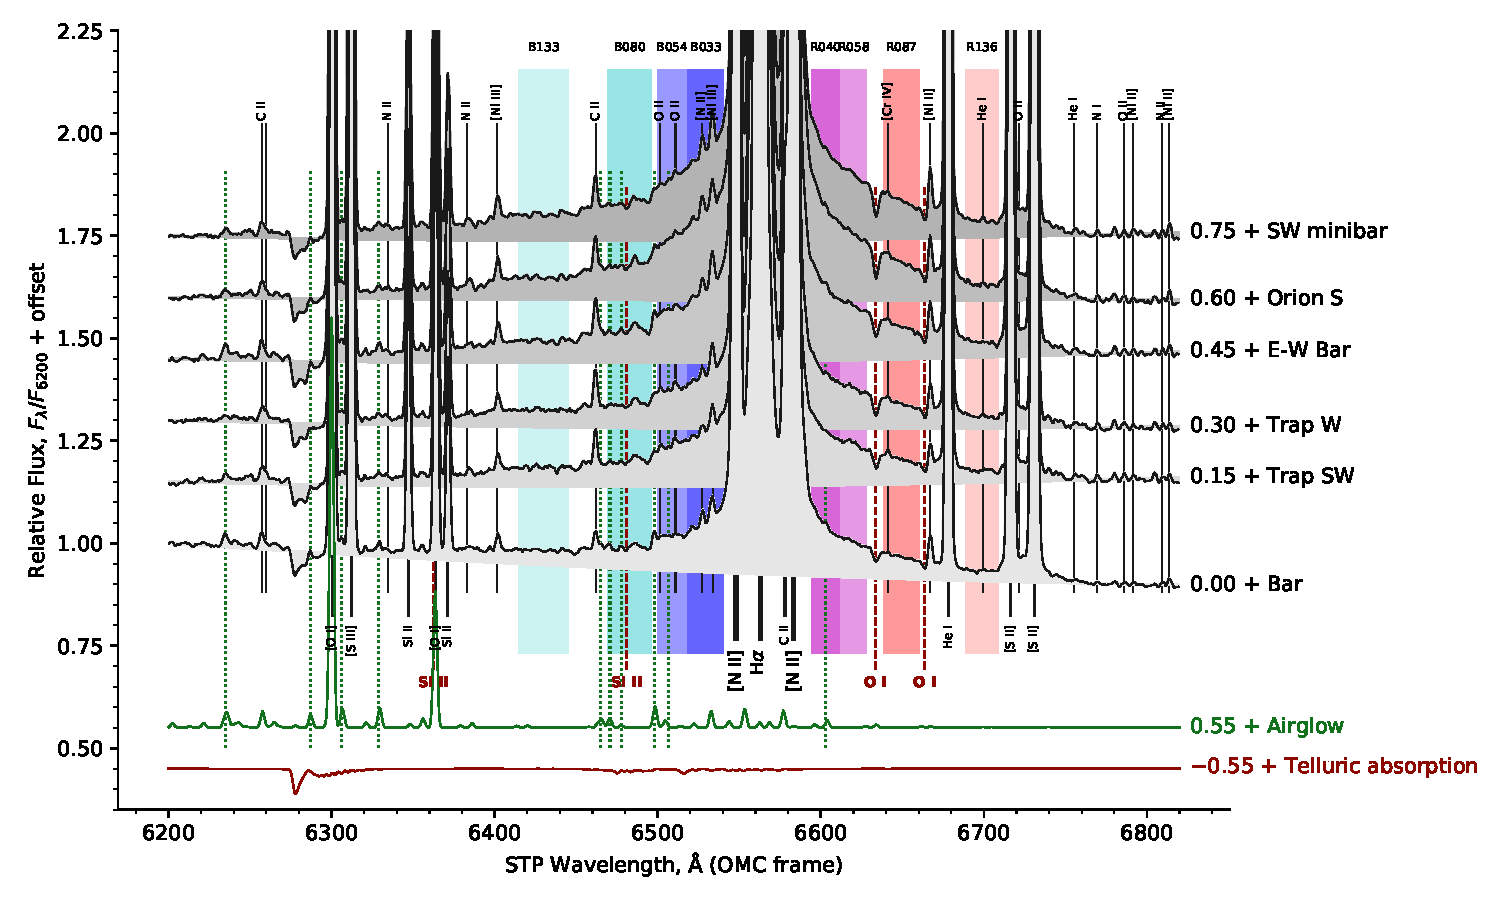
\includegraphics[width=\linewidth]{figs/raman-orion-muse-1d-spectra}
  \caption{MUSE spectra centered on the H\(\alpha\) line, showing the broad
    Raman-scattered wings.}
  \label{fig:raman-spectra-1d}
\end{figure*}

\begin{figure*}
  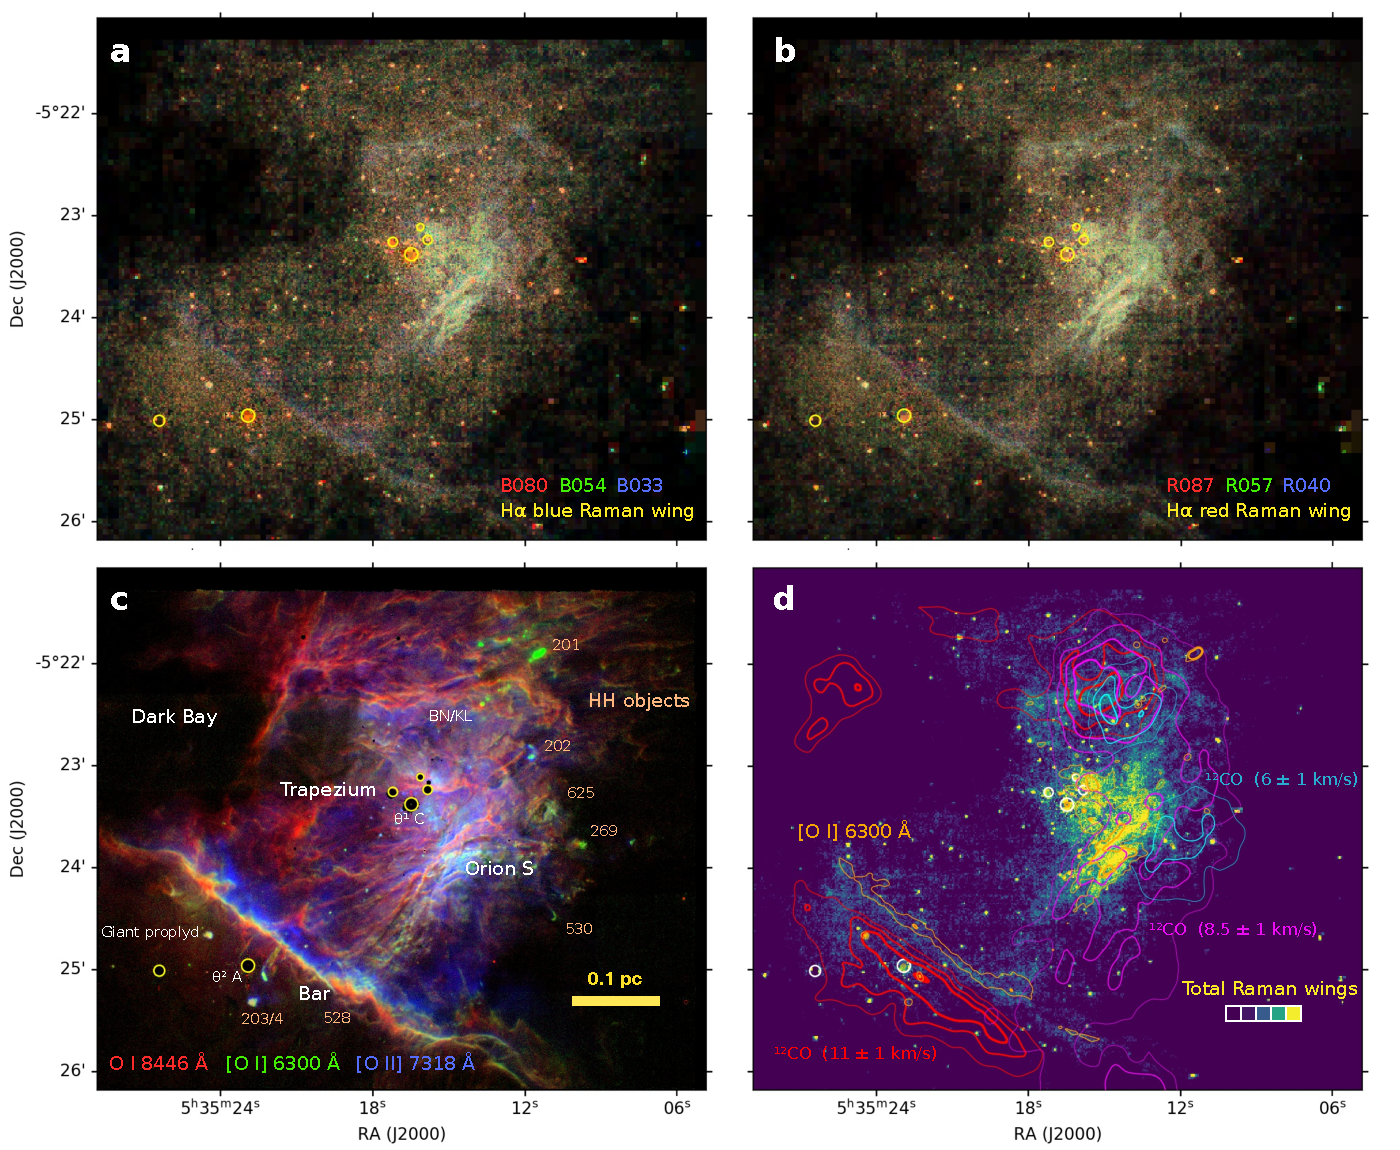
\includegraphics[width=\linewidth]{figs/raman-rgb-4-panel}
  \caption{Spatial distribution of Raman-scattered wings in H\(\alpha\)}
  \label{fig:raman-maps}
\end{figure*}

MUSE \citep{Bacon:2010a} observations of the Orion Nebula \citep{Weilbacher:2015a, Mc-Leod:2015b}.


The bands are chosen to avoid the stronger sky lines (e.g.,
\SI{6498}{\angstrom}) and nebula lines (e.g., ), but some weak line
contamination remains, as listed in the last column of
Table~\ref{tab:wav-bands}.


\section{Raman scattering of spectral lines}
\label{sec:raman-scatt-spectr}

When a photon is Raman-scattered from the vicinity of \lyb{} (UV
domain) to the vicinity of \ha{} (optical domain) its wavelength is
transformed from \(\lambda_1\) to \(\lambda_2\).  Intervals in frequency
(\(\nu = c/\lambda\)) or wavenumber (\(\wn = 1 / \lambda\)) space are conserved
between the two domains. For example the wavenumber displacement from
the \ion{H}{1} line center can be written in two ways:
\begin{equation}
  \label{eq:delta-wavnum}
  \Delta\wn = \wn_1 - \wn(\lyb) = \wn_2 - \wn(\ha) \ ,
\end{equation}
from which it follows that
\begin{equation}
  \label{eq:wav-transform}
  \lambda_2 = \left( \frac1{\lambda(\ha)} +\frac1{\lambda_1} - \frac1{\lambda(\lyb)}\right)^{-1} \ .
\end{equation}
The wavelengths \(\lambda(\lyb)\) and \(\lambda(\ha)\), together with their
corresponding wavenumbers, are given in Table~\ref{tab:line-fits} (all
wavelengths are on the vacuum scale unless otherwise noted).  For both
lines, a weighted average over the \Level{3p}{2}{P}{1/2} and
\Level{3p}{2}{P}{3/2} upper levels is used, assumed to be populated
according to their statistical weights, with individual component
wavelengths obtained from Tab.~XXVIII of \citet{Mohr:2008a}. Note that
the electric dipole selection rules mean that only \Config{3p \to 2s}
transitions contribute to \ha{} in the Raman scattering context.  The
wavelength is therefore slightly shorter than the value obtained for
the \ha{} recombination line, which includes additional contributions
from \Config{3s \to 2p} and \Config{3d \to 2p}. The shift is of order
\SI{-0.05}{\angstrom} or \SI{-2}{km.s^{-1}} with respect to the Case~B
results reported in Tab.~6a of \citet{Clegg:1999a}.

Also listed in Table~\ref{tab:line-fits} are the Raman transformations
\(\lambda_1 \to \lambda_2\) for the rest wavelengths of transitions between the
ground \Term{2s^2 2p^4}{3}{P} term of neutral \chem{^{16}O} and the
excited \Term{2s^2 2p^3 3d}{3}{D^o} term. The \ion{O}{1} data is obtained
from highly accurate laser metrology \citep{Ivanov:2008a,
  Marinov:2017a}, with a precision of \SI{0.08}{cm^{-1}} or better.
The fine structure splitting between the \(J_k\) levels of the excited
term (\(\sim \SI{0.1}{cm^{-1}}\)) is much smaller than that between the
\(J_i\) levels of the ground term (\(\sim \SI{100}{cm^{-2}}\)), so that
the 6 transitions fall into 3 well-separated groups.  The three
transitions from the lowest energy \(J_i=2\) level are very close to
\lyb{} (\(\Delta\wn \approx \SI{4}{cm^{-1}}\)), whereas the two transitions from
\(J_i=1\) (\(\Delta\wn \approx \SI{162}{cm^{-1}}\)) and the single transition
from \(J_i=0\) (\(\Delta\wn \approx \SI{231}{cm^{-1}}\)) lie increasingly to the
red.  The corresponding wavelengths in the optical domain,
\(\lambda_2\), are therefore on the red side of \ha{}.  The final column of
the table uses STP refractive indices \citep{Greisen:2006a} to convert
\(\lambda_2\) to air wavelengths, \(\lambda_{\text{air}}\), for ease of comparison
with ground-based optical spectroscopy.  The resultant wavelength is
\SI{6663.747}{\angstrom} for the line from \(J_i = 0\), with an
uncertainty of about \SI{0.004}{\angstrom}, which is much smaller than
typical observational precision (for instance, \SI{0.07}{\angstrom}
for a very high resolution spectrograph with resolving power of
\(R = \num{e5}\)). The two lines from \(J_i = 1\), with a separation
of \SI{0.028}{\angstrom}, will always be blended in observations,
giving a mean wavelength of \SI{6633.347}{\angstrom} (assuming the
upper levels are distributed according to statistical weight
\(2 J_k + 1\)).  Similarly, the three lines from \(J_i = 2\) have a
mean wavelength of \SI{6564.386}{\angstrom}, but this is so close to
\ha{} (corresponding to a Doppler shift of \SI{+75}{km.s^{-1}}) that
it would be very difficult to observe.

The \SI{6633}{\angstrom} and \SI{6664}{\angstrom} lines are clearly
detected in the MUSE spectra as absorption features against the
pseudo-continuum of the broad \ha{} wings (see Fig~XX), although the
latter is blended with a \ion{Ni}{2} emission line at
\SI{6666.8}{\angstrom}.  This is further proof of the Raman scattering
nature of the wings.


\section{High-resolution spectroscopy of Raman-scattered \ion{O}{1} \SI{1028}{\angstrom}}
\label{sec:keck-observations}


Keck HIRES spectra described in \citet{Henney:1999a} and
\citet{Bally:2000a}. The spectrum I use is of HH~529 base region in
Orion~South. Published results from these data have concentrated on
strong nebular lines, but here I use a small section of the spectrum
in the range \SIrange{6660}{6670}{\angstrom} for reasons which will
become apparent.


\begin{figure*}
  \centering
  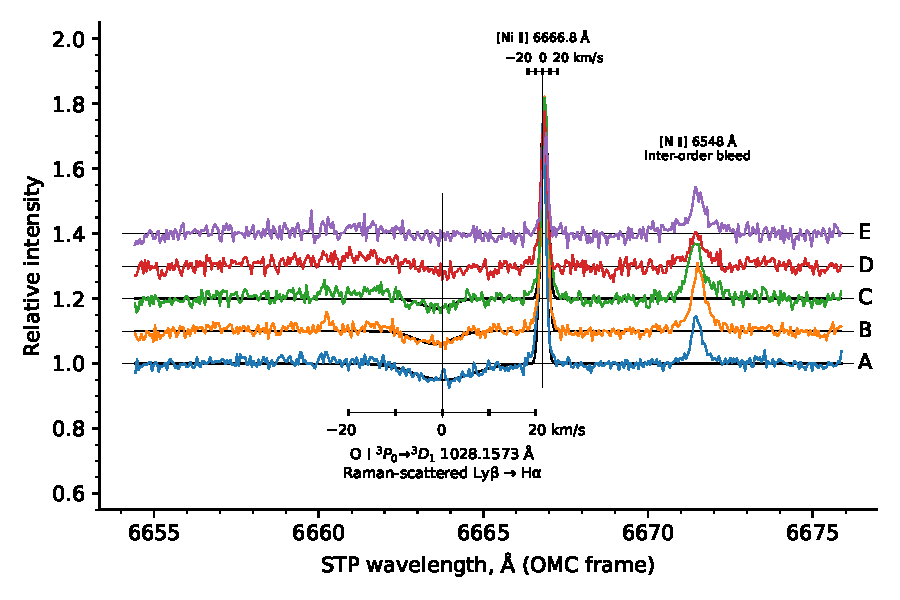
\includegraphics[width=\linewidth]{figs/order51-absorption-by-group}
  \caption{Keck HIRES spectra of Raman-scattered \ion{O}{1} absorption
    line for five regions in Orion~South.  Wavelengths are given on an
    air scale and in the rest-frame of the Orion Molecular Cloud, as
    defined by the peak velocity of \chem{^{13}CO}. }
  \label{fig:raman-keck}
\end{figure*}


\begin{table*}
  \caption{FUV/optical wavelength equivalencies for Raman scattering}
  ~\\[-\baselineskip]
  \begin{tabular}{L L L C C R C C C}\toprule
    % Transition & {UV wav, \AA{}} & {Freq, cm\textsuperscript{-1}} & {d Freq} & {Opt wav} & {Air wav}\\
    \text{Ion} & \text{Transition} & J_i \to J_k & \lambda_1,\ \si{\angstrom} & \wn_1,\ \si{cm^{-1}} & \Delta\wn,\  \si{cm^{-1}}& \wn_2,\ \si{cm^{-1}} & \lambda_2,\ \si{\angstrom} & \lambda_{\text{air}},\ \si{\angstrom} \\
    \midrule
    & & & \multicolumn{2}{c}{\dotfill\(\quad \lyb,\ n = 1 \quad\)\dotfill} & & \multicolumn{3}{c}{\dotfill\(\quad \ha,\ n = 2 \quad\)\dotfill} \\
    \addlinespace[2pt]
    \ion{H}{1} & n\Term{s}{2}{S} \to \Term{3p}{2}{P} & \tfrac12 \to \tfrac12,\tfrac32 & 1025.72220 & 97492.283 & 0.000 & 15233.329 & 6564.553 & 6562.740\\
    \addlinespace
    \ion{O}{1} & \Term{2s^2 2p^4}{3}{P}  \to \Term{2s^2 2p^3 (^4S) 3d}{3}{D^o} & 0 \to 1 & 1028.15729 & 97261.383 & -230.900 & 15002.429 & 6665.587 & 6663.747\\
     & & 1 \to 1 & 1027.43139 & 97330.100 & -162.183 & 15071.146 & 6635.196 & 6633.364\\
     & & 1 \to 2 & 1027.43077 & 97330.159 & -162.124 & 15071.205 & 6635.170 & 6633.338\\
     & & 2 \to 1 & 1025.76339 & 97488.369 & -3.914 & 15229.415 & 6566.240 & 6564.427\\
     & & 2 \to 2 & 1025.76276 & 97488.429 & -3.854 & 15229.475 & 6566.215 & 6564.401\\
     & & 2 \to 3 & 1025.76170 & 97488.530 & -3.753 & 15229.576 & 6566.171 & 6564.358\\
    \bottomrule
  \end{tabular}
\end{table*}

\begin{table}
  \caption{Fit parameters from Gaussian line fits}
  \label{tab:line-fits}
  \begin{tabular}{l RRR RRR}\toprule
     & \multicolumn{3}{c}{\ion{O}{1}} & \multicolumn{3}{c}{\ion{Ni}{2}} \\
    Region & A & V & \sigma & A & V & \sigma \\ \midrule
    A & & & & & & \\
    B & & & & & &  \\
    C & & & & & &  \\
    D & & & & & &  \\
    E & & & & & &  \\ \bottomrule
  \end{tabular}
\end{table}

\section{Discussion}
\label{sec:discussion}

The effective resolving power of the optical spectrograph is multiplied by 6.4 for the FUV domain.

The \ion{O}{1} lines should be in absorption in the spectrum seen by the Raman scatterers. 

\citet{Salgado:2016a} had found low dust cross-section in Orion Bar
PDR, but there are loopholes. First, they assume plane-parallel
geometry with exactly edge-on viewing angle, while in reality it is a
roughly cylindrical filament.  Second, they ignore scattering, see
\citet{Watson:1998a}.

Non-equilibrium PDRs \citep{Stoerzer:1998a, Bertoldi:1996a}.  Recent models from \citet{Bron:2018a}. 

\ion{C}{1} emission from non-steady PDRs \citep{Stoerzer:1997a} (fine structure lines, but maybe optical lines would be similar).  \citet{Escalante:1991a} model the far-red [\ion{C}{1}] line as recombination of \chem{C^+}.


Geometry of bar: in \citet{Henney:2005b} I pointed out that a
diverging cylindrical geometry is necessary to explain the sharp peak
in the [\ion{N}{2}] emissivity seen at the ionization front.  It has
been apparent since \citet{ODell:2000a} that the nebula contains many
bar-like features.

Even for high PDR optical depth, no multiple Raman scattering will
occur since the population of \(2s\) is very small and the
post-scattered photons have insufficient energy to excite any
transitions from \(1s\).



\acknowledgments
This work has made use of the Atomic Line List\footnote{\url{https://www.pa.uky.edu/~peter/newpage/}} \citep{Van-Hoof:2018a}. 


\bibliography{BibdeskLibrary}


\end{document}


\end{document}
%%% Local Variables:
%%% mode: latex
%%% TeX-master: t
%%% End:
